
\chapter{Web Technologies}
\label{chap:WebTechnologies}

RespVis is a web-based framework. As such, it builds on a stack of
technologies which are native to the web. The first sections in this
chapter introduce the web's core technologies: HTML for content, CSS
for presentation, and JavaScript (JS) for behavior. Next, TypeScript
is introduced, and the different technologies to embed graphics in web
pages are discussed. Due to the importance of layouting in this work,
three different forms of layout engines are compared. Finally, the
concept of responsive web design is summarized. Since there are many
things to examine, none of the following sections goes into great
detail, the aim is to give a summary of the concepts that are
introduced. For more in-depth information, works referenced in the
sections below should be consulted.


\section{HyperText Markup Language (HTML)}
\label{sec:HTML}

HTML is a document markup language for documents which are to be
displayed in web browsers. The original proposal and implementation in
1989 came from Tim Berners-Lee who was a contractor at CERN at the
time \parencite{TBLProposal}. Over the years, the standard was further
developed by a range of different entities like the CERN and the
Internet Engineering Task Force (IETF). Nowadays, HTML exists as a
continuously evolving living standard without specific version
releases, which is maintained by the Web Hypertext Application
Technology Working Group (WHATWG) and the World Wide Web Consortium
(W3C) \parencite{HTML}.

The primary purpose of HTML is to define the content and structure of
web pages. This is achieved with the help of HTML elements, such as
\elname{<section>}, \elname{<h1>}, \elname{<p>}, and \elname{<img>},
which are composed into a hierarchical tree structure of modular
content, and which is then interpreted by web browsers. A strong
pillar of HTML's design is extensibility. There are multiple
mechanisms in place to ensure its applicability to a vast range of use
cases, including:
\begin{itemize}
\item Specifying classes of elements using the \attrname{class}
  attribute. This effectively creates custom elements based on the
  closest standard elements.

\item Using \attrname{data-*} attributes to decorate elements with
  additional data which can be used by scripts. The HTML standard
  guarantees that these attributes are ignored by browsers.

\item Embedding custom data using \elname{<script type="">} elements,
  which can be accessed by scripts.
\end{itemize}





\section{Cascading Style Sheets (CSS)}
\label{sec:CSS}

Cascading Style Sheets (CSS) apply styling to HTML elements,
effectively separating presentation from content. In earlier versions
of HTML \parencite{HTML32}, elements like \elname{<strong>} and
\elname{<em>} muddied the boundary between presentation and content.

A CSS style sheet can either be embedded directly in HTML documents
using a \elname{<style>} element or can be defined externally and
linked to using a \elname{<link>} element. This characteristic of
being able to externally describe the presentation of documents brings
great flexibility because multiple documents with different content
can reuse the same presentation by linking to the same CSS file.
Conversely, alternative style sheets can be applied to the same HTML
content to achieve a different styling.

CSS was initially proposed by \textcite{CSSProposal} and standardized
into CSS1 by the W3C in 1996 \parencite{CSS1}. Throughout its history,
the adoption of CSS by browser vendors was fraught with complications
and even though most major browsers soon supported almost the full CSS
standard, their implementations sometimes behaved differently. This
meant that authors of web pages often had to resort to workarounds,
including providing different style sheets for different browsers. In
recent years, CSS specifications have become much more detailed
\parencite{CSS21} and browser implementations have become more stable
with fewer inconsistencies. It has therefore become much rarer that
browser-specific workarounds need to be applied, dramatically
improving the developer experience. CSS 2.1 \parencite{CSS21} was the
last CSS standard published as a single, monolithic
specification. Since then, the specification has been modularized into
different documents \parencite{CSSSnapshot2020}, each describing a
specific module of the overall CSS specification.
 

A CSS style sheet contains a collection of rules. Each rule consists
of a selector and a block of style declarations. Selectors are defined
in a custom syntax and are used to match HTML elements.  All elements
which are matched by the selector of a rule will have the rule's style
declarations applied to them. The selector syntax is fairly
straightforward when selecting elements of a certain type, but also
has more sophisticated mechanisms for selecting elements based on
their contexts or attributes. Table~\ref{tab:CSSSelectorSyntax}
summarizes the selector syntax of CSS Selectors Level 3
\parencite{CSSSelectors3}.




\begin{table}[tp]
\tablestretch
\rowcolors{2}{}{tablerowcolour}
\centering
\begin{tabularx}{\linewidth}{>{\kern-\tabcolsep}lX<{\kern-\tabcolsep}}
\toprule
Pattern & Matches \\
\midrule
\pattname{*}      & Any element. \\
\pattname{E}      & Elements of type E. \\
\pattname{E F}    & Any element of type F which is a descendant of elements of type E. \\
\pattname{E > F}  & Any element of type F which is a direct descendant of elements of type E. \\
\pattname{E + F}  & Any element of type F which is a directly preceded by a sibling element of type E. \\
\pattname{E:P}    & Elements of type E which also have the pseudo class P. \\
\pattname{.C}     & Elements which have the class  C. \\
\pattname{#I}     & Elements which have the ID I. \\
\pattname{[A]}    & Elements which have an attribute A. \\
\pattname{[A=V]}  & Elements which have an attribute A with a value of V. \\
\pattname{S1, S2} & Elements which match either the selector S1 or the selector S2. \\
\bottomrule
\end{tabularx}
\caption[CSS Selector Syntax]{
A summary of the CSS 2.1 selector syntax.
\imgcredit{Table created by the author of this thesis with data from \parencite{CSSSelectors3}.}
}
\label{tab:CSSSelectorSyntax}
\end{table}


Another important characteristic of CSS is the cascading of styles.
The exact rules for calculating the final style to be applied to an
element are quite involved, and \textcite{CSSCascading3}
should be consulted for a detailed description. The most important
aspect in the context of this work is that styles can be
overwritten. When multiple rules match an element and define different
values for the same property, the values of the rule with higher
specificity will be applied. If multiple rules have the same
specificity, the one defined last in the document tree will overwrite
all previous ones.





\subsection{CSS Box Model}
\label{sec:BoxLayout}

All elements in an HTML document are laid out as boxes. The CSS box
model specifies how every element is wrapped in a rectangular box and
every box is described by its content and optional surrounding margin,
border, and padding areas. Margins are used to specify invisible
spacing between boxes. The border provides a visible frame around the
content of a box. The padding provides invisible spacing between the
content and the border. A visual representation of these properties
can be seen in Figure~\ref{fig:BoxModel}.

\begin{figure}[tp]
\centering
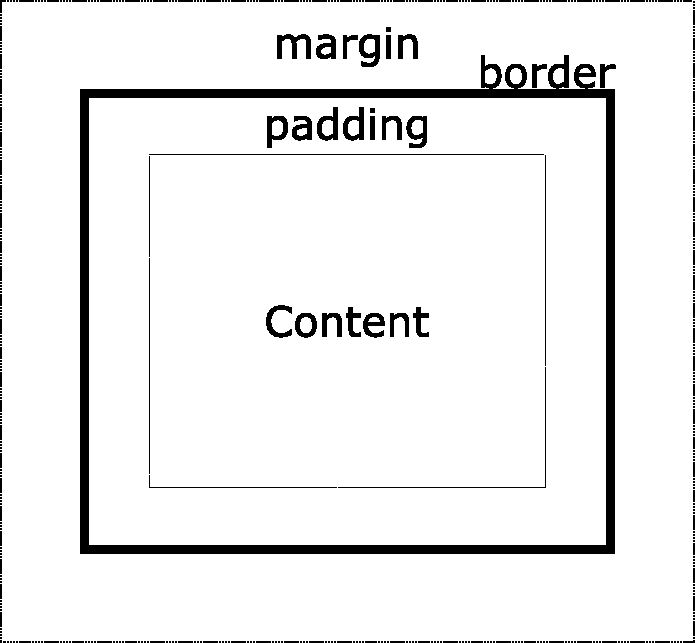
\includegraphics[keepaspectratio,width=\linewidth,height=\thirdh]
{diagrams/box-model.pdf}
\caption[CSS Box Model]{
The CSS box model defines the properties of boxes which wrap around HTML elements.
\imgcredit{Image drawn by the author of this thesis.}
}
\label{fig:BoxModel}
\end{figure}

In early versions of CSS, before the introduction of the Flexible Box
(Flexbox) layout module \parencite{CSSFlexboxFirstDraft}, the box
model was the only way to lay out elements. Style sheet authors had to
meticulously define margins of elements and their relative (or
absolute) positions in the document tree. The responsive capabilities
of this kind of layouting were very limited, because different
configurations for varying screen sizes had to be specified manually
using media queries. More complex features, like the filling of
available space, required manual implementation via scripting.





\subsection{CSS Flexbox Layout}
\label{sec:Flexbox}

CSS Flexible Box layout (Flexbox) \parencite{CSSFlexbox} is a
mechanism for one-dimensional layout of elements in either rows or
columns. This one-dimensionality is what separates it from grid-based
layout, which is inherently two-dimensional.
%
Even though the first draft of the Flexbox layout module was already
published in 2009 \parencite{CSSFlexboxFirstDraft}, implementations by
browser vendors have been a slow and bug-ridden process
\parencite{CanIUseCSSFlexbox}, which held back adoption by users for
several years after its inception. More recently though, partly
through the deprecation of Internet Explorer
\parencite{IEDeprecation}, all major browsers have mature
implementations of current Flexbox standards \parencite{CSSFlexbox},
and, in most cases, fallback styling is no longer necessary.

Flexbox layouting is enabled for child elements by setting the CSS
\cssname{display} property to \code{flex} on a container element. The
direction of the layout can then be specified using the CSS
\cssname{flex-direction} property which can be set to either
\code{row} or \code{column}.
%
The items inside a Flexbox container can have either a fixed or a
relative size. When items should be sized relative to the size of
their containers, the proportions of how the available space should be
divided can be controlled using ratios. These ratios can be set on
item elements via the CSS \cssname{flex} property.

Another important feature of Flexbox layout is the controllable
spacing of items, which can be specified separately for both the main
axis and the cross axis of the layout. Spacing along the main axis can
be configured with the CSS \cssname{justify-content} property, which
can take a number of different values and is illustrated in
Figure~\ref{fig:FlexboxJustifyContent}. Alignment of items on the
cross axis is achieved either by the CSS \cssname{align-items}
property on the container element or the CSS \cssname{align-self}
property on the items themselves.

\begin{figure}[tp]
\centering
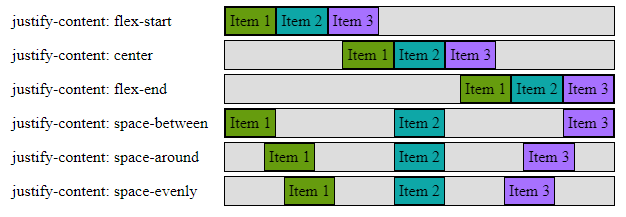
\includegraphics[keepaspectratio,width=\linewidth,height=\thirdh]
{images/flexbox-justify-content.png}
\caption[Flexbox CSS \cssname{justify-content} Property]{
The CSS \cssname{justify-content} property is used to distribute
items along the main axis of a Flexbox container. 
\imgcredit{Image created by the author of this thesis.}
}
\label{fig:FlexboxJustifyContent}
\end{figure}


This section only grazed the surface of what is possible with the
Flexbox layout module. There are many more useful CSS properties like
\cssname{flex-grow}, \cssname{flex-shrink}, and \cssname{flex-wrap}.
For a more detailed look at this topic it is recommended to review the
specification \parencite{CSSFlexbox} and read the excellent tutorial
by Chris Coyier \parencite{Coyier-FlexboxGuide}.





\subsection{CSS Grid Layout}
\label{sec:Grid}

The CSS Grid Layout Module \parencite{CSSGrid} defines the layout of
elements in a two-dimensional grid. The initial proposal of the CSS
Grid layout module was published in 2011 \parencite{CSSGridFirstDraft}
and has been further refined over the years. At the time of writing,
even though it still exists as merely a candidate recommendation for
standardization \parencite{CSSGrid}, many browsers have already
adopted it. Similar to the adoption of Flexbox, the history of browser
adoption of CSS Grid was initially strewn with inconsistencies and
bugs. However, in 2017 the major browsers Chrome, Firefox, Safari, and
Edge removed the need for vendor prefixes and implementations are now
considered stable \parencite{CanIUseCSSGrid}.

Grid layout of elements is enabled by setting the CSS
\cssname{display} property to \code{grid} on their container. The grid
in which items shall be laid out is then defined using the CSS
\cssname{grid-template-rows} and \cssname{grid-template-columns}
properties. In addition, the CSS \cssname{grid-template} property can
be used as a shorthand to simultaneously specify both the rows and
columns of a grid.
%
Item elements need to specify the cell of the grid into which they
shall be positioned. This is done with the CSS \cssname{grid-row} and
\cssname{grid-column} properties, which take the corresponding row and
column indices as values. Items can also be configured to span
multiple cells by specifying index ranges as the values of those
properties.

Every cell in a grid can also be assigned a specific name via the CSS
\cssname{grid-template-areas} property on the grid container element.
The items within the grid can then position themselves in specifically
named grid cells using the CSS \cssname{grid-area} property instead of
directly setting the row and column indices. The benefit of
positioning items this way is that the structure of the grid can be
freely changed without having to respecify the cells in which items
belong. As long as the new layout still specifies the same names of
cells somewhere in the grid, the items will be automatically placed at
their new positions.

There are also properties which control the layout of items within
grid cells and the layout of grid cells themselves. Similar to
Flexbox, this can be configured with the CSS \cssname{align-items} and
\cssname{justify-items} properties for laying out within grid cells,
and the CSS \cssname{align-content} and \cssname{justify-content}
properties for laying out the grid cells themselves. The latter
\cssname{*-content} properties only make sense when the cells do not
cover the full area of the grid. For a visual comparison between the
\cssname{*-items} and \cssname{*-content} properties, see
Figure~\ref{fig:GridLayoutProperties}.


\begin{figure}[tp]
\centering
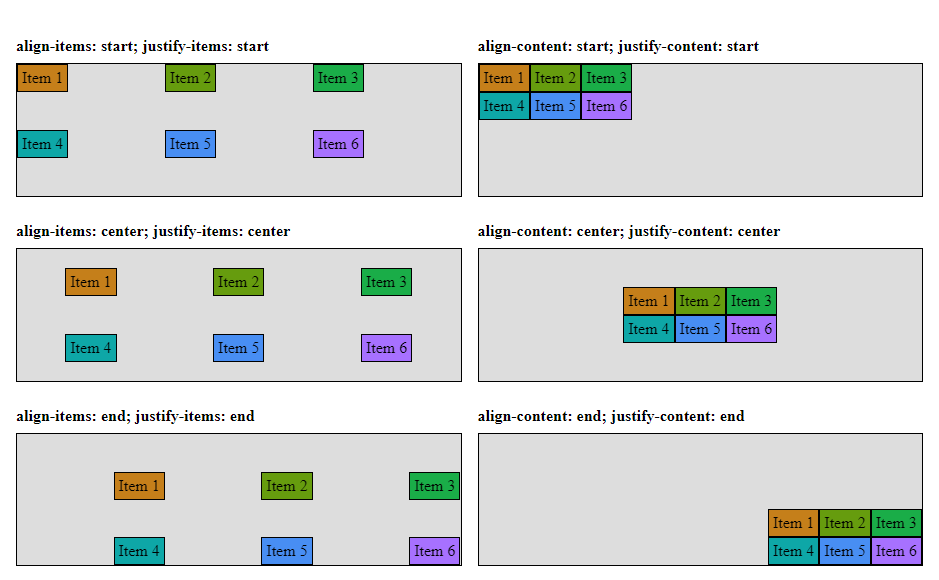
\includegraphics[keepaspectratio,width=\linewidth,height=\halfh]
{images/grid-layout-properties.png}
\caption[Grid Layout Property Comparision]{
The \cssname{*-items} properties are used to lay out items within
their grid cells, whereas the \cssname{*-content} properties are
used to lay out the grid cells themselves. 
\imgcredit{Image created by the author of this thesis.}
}
\label{fig:GridLayoutProperties}
\end{figure}


There is some apparent overlap between the CSS Grid and Flexbox layout
modules. At first sight, it seems like Grid layout supersedes Flexbox
layout, because everything which can be done using Flexbox layout can
also be done with Grid layout. While that is true, the inherent
difference in dimensionality and the resulting syntactic
characteristics lead to better suitability of one technology over the
other, depending on the context of use. As a general rule
\parencite{CSSGridVsFlexbox}, top-level layouts which require
two-dimensional positioning of elements are usually best implemented
using a Grid layout, whereas low-level layouts which merely need
laying out on a one-dimensional axis are better implemented using a
Flexbox layout.

For more details, the CSS Grid specification \parencite{CSSGrid} and
other sources like \textcite{GridLayoutInCSS} and
\textcite{House-GridGuide} are recommended.




\section{JavaScript (JS)}
\label{sec:JS}

JavaScript was originally developed as a client-side scripting
language run by an interpreter (engine) inside the web browser.
Nowadays, there are also standalone JavaScript engines and
environments like NodeJS \parencite{NodeJS}. JavaScript is a
multi-paradigm language which supports event-driven, as well as
functional and imperative programming. Driven by the popularity of the
web, JavaScript is currently the most used programming language
worldwide \parencite{StatisticProgrammingLanguageUsage}.

JavaScript was initially created by Netscape in 1995
\parencite{JSFirstRelease}. Before that, websites were only able to
display static content, which drastically limited the usefulness of
the web. Microsoft seemingly saw JavaScript as a potentially
revolutionary development, because they reverse-engineered Netscape's
implementation and published their own version of the language for
Internet Explorer in 1996 \parencite{JSIERelease}. The two
implementations were noticeably different from one another and the
uncontested monopoly of the Internet Explorer
\parencite{BrowserMarketShareEarly} held back standardization efforts
undertaken by Netscape \parencite{ECMAScript1}. When Firefox was
released in 2004 \parencite{FirefoxFirstRelease} and Chrome in 2008
\parencite{ChromeFirstRelease}, they quickly gained a considerable
share of the market \parencite{BrowserMarketShare}, as shown in
Figure~\ref{fig:BrowserMarketShare}. Galvanized by this new market
reality, all major browser vendors collaborated on the standardization
of JavaScript as ECMAScript 5 in 2009 \parencite{ECMAScript5}. Since
then, JavaScript has been continuously developed and its later
versions ECMAScript 2015 to 2021
\parencite{ECMAScript6, ECMAScript7, ECMAScript8, ECMAScript9, ECMAScript10, ECMAScript11, ECMAScript12}
are widely supported.


\begin{figure}[tp]
\centering
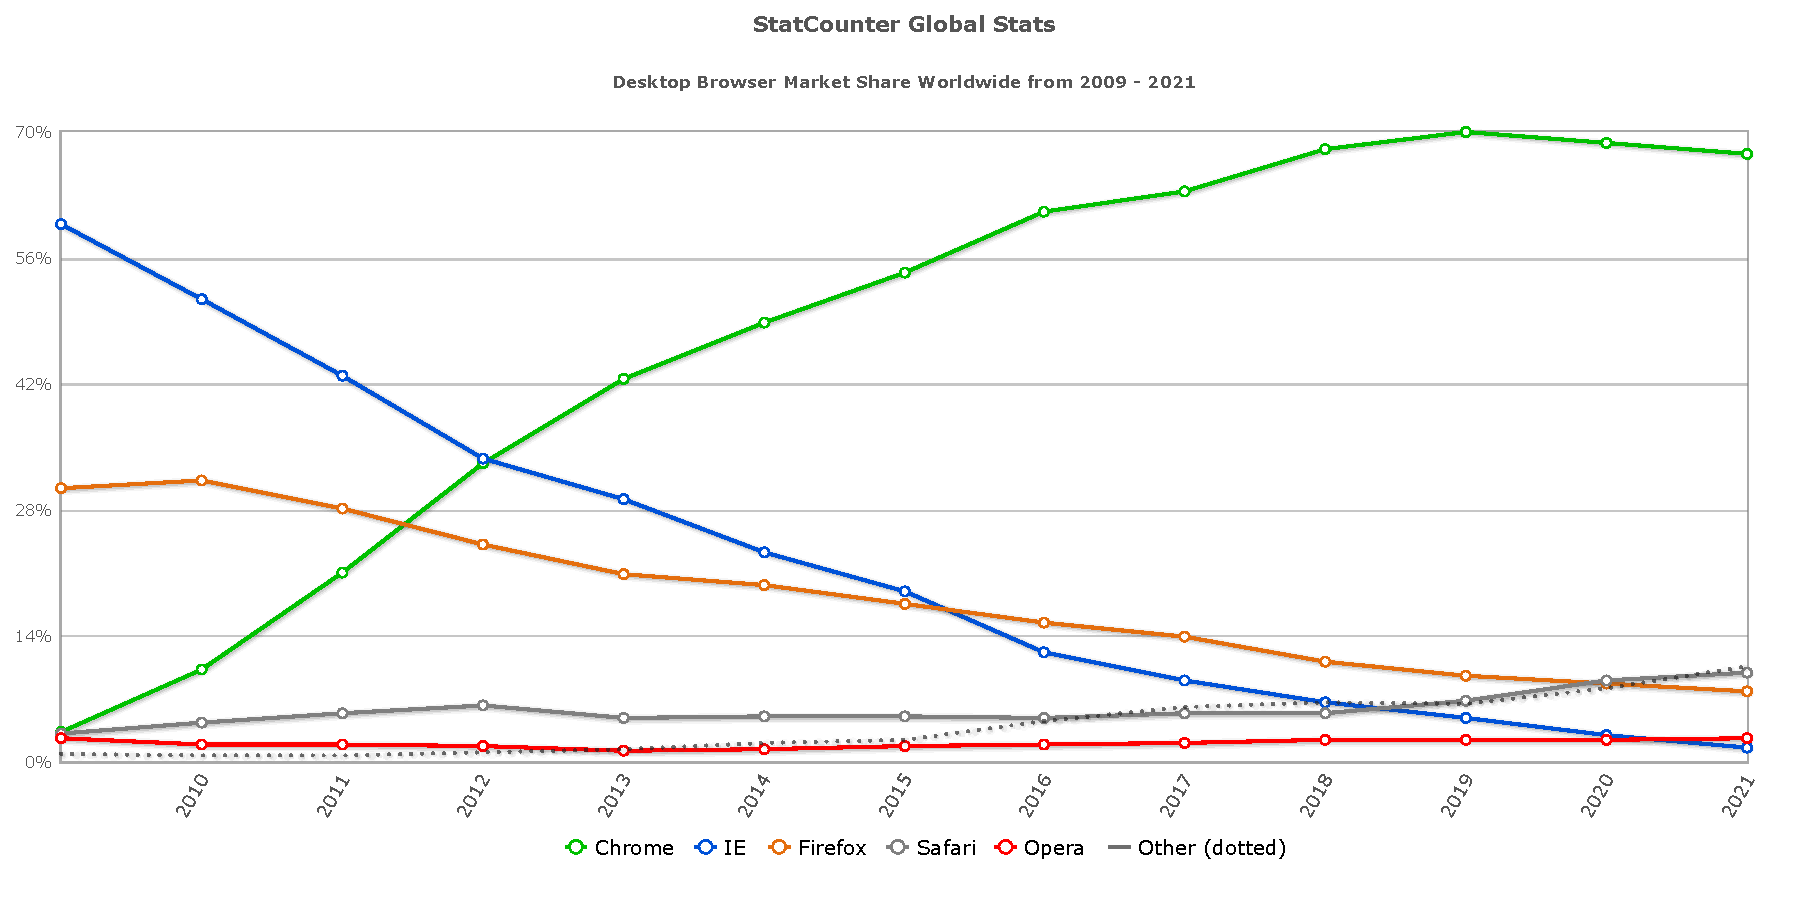
\includegraphics[keepaspectratio,width=\linewidth,height=\fullh / 3]{diagrams/browser-market-share.pdf}
\caption[Desktop Browser Market Share]{
  Since their release, Firefox and Chrome have contested the monopoly of the Internet Explorer and continuously gained more market share. 
  Recently, Chrome seems to be gaining an increasingly strong position within the market. 
  \imgcredit{Image taken from \textcite{BrowserMarketShare}}}
\label{fig:BrowserMarketShare}
\end{figure}


RespVis is a browser-based library which is designed to run within the
JavaScript engine of a browser. It builds heavily on widely supported
Web APIs, which are JavaScript modules specifically meant for
development of web pages. These Web APIs are standardized by the W3C
and each browser has to individually implement them in their
JavaScript engine.

The most popular Web API, which every web developer is familiar with,
is the Document Object Model (DOM). The DOM is the programming
interface and data representation of a web page or document.
Internally, a document is modeled as a tree of objects, where each
object corresponds to a specific HTML or SVG element in the document
hierarchy and its associated data and functions. In addition to the
querying of elements, the DOM also defines functionality to mutate
them and their attributes, as well as functionality for handling and
dispatching events. It also exposes the mechanism of
\modname{MutationObservers}, which are used to observe changes of
attributes and children in the document tree. The initial
specification of the DOM was published in 1997 \parencite{DOM1}. It
is currently maintained as a living standard by the WHATWG
\parencite{DOM}.

Another important Web API in the context of this work is the
\modname{ResizeObserver} API. It provides the ability to observe an
element's size and respond to changes, which increases the responsive
capabilities of websites. Previously, scripts could only respond to
changes in the overall viewport size via the \code{resize} event
on the \code{window} object, but this meant that changes of an
individual element's size through attribute changes could not be
detected. This limitation is fixed with the \modname{ResizeObserver}
API, which is already fully supported by all modern browsers, even
though it has so far only been published as an editor's draft
\parencite{ResizeObserver}.






\section{TypeScript (TS)}
\label{sec:TS}

TypeScript (TS) is a strongly-typed programming language which is
designed as an extension of JavaScript. Syntactically, it is a
superset of JavaScript which enables the annotation of properties,
variables, parameters, and return values with types. It requires a
transpiler (compiler) to convert the TypeScript code into valid
JavaScript code for a specific ECMAScript version.

Initially, TypeScript was released by Microsoft in 2012
\parencite{TSFirstRelease} to extend JavaScript with features which
were already present in more mature languages, and whose absence in
JavaScript caused difficulties when working on larger codebases. At
the time of TypeScript's initial development, it provided features
which would later be offered by ECMAScript 6, including a module
system to be able to split source code into reusable chunks and a
class system to aid object-oriented development. TypeScript code using
these features could then be transpiled into standard-conformant
JavaScript code, which could be interpreted by JavaScript engines of
the time. At the time of writing, ECMAScript 6 is widely supported by
all modern browsers and therefore the main benefit of TypeScript over
JavaScript lies in its provision of a static type system.

The extension of JavaScript with a static type system brings many
benefits, including the improved tooling which comes with
type-annotated code. Tools such as linters \parencite{ESLint} are able
to point out errors early in development and assist developers with
automated fixes, improved code completion, and code navigation.
Additionally, studies like \textcite{ToTypeOrNotToType} looked at
software bugs in publicly available codebases and found that 15\% of
them could have been prevented with static type checking.

The TypeScript type system was designed to support JavaScript
constructs as completely as possible, via structural types and unified
object types. Another goal was to make the type annotation of
JavaScript code as effortless as possible to improve adoption by
existing projects. This was done by consciously allowing the type
system to be statically unsound via gradual typing and also by
employing type inference to reduce the number of necessary
annotations. The major properties of TypeScript's type system design
are summarized in Table~\ref{tab:TSTypeSystemDesignProperties}.


\begin{table}[tp]
\tablestretch
\rowcolors{2}{}{tablerowcolour}
\centering
\begin{tabularx}{\linewidth}{>{\kern-\tabcolsep}lX<{\kern-\tabcolsep}}
\toprule
Design Property & Description \\
\midrule
Full erasure         &
Types are completely removed by the compiler, there is no type checking at runtime. \\
%
Type inference       &
Many types can be inferred from usage, minimizing the number of types which have to be explicitly stated. \\
%
Gradual typing       &
Type checking can be selectively prevented using the dynamic type \lstinline{any}. \\
%
Structural types     &
Types are defined via their structure as opposed to via their names.
This better fits JavaScript, where objects are usually custom-built and used based on their shapes. \\
%
Unified object types &
A type can simultaneously describe objects, functions, and arrays.
These constructs are common in JavaScript and thus TypeScript needs to support their typing. \\
\bottomrule
\end{tabularx}
\caption[TypeScript Type System Design Properties]{
A summary of the major design properties on which TypeScript's type system is built.
\imgcredit{Table created by the author of this thesis with data from \textcite{UnderstandingTS}.}
}
\label{tab:TSTypeSystemDesignProperties}
\end{table}









\section{Web Graphics}
\label{sec:WebGraphics}

Graphics are used as a medium for visual expression to enhance the
representation of information on the web. There are many fields of
application like the integration of maps, photographs, or charts in a
web page. Multiple complementary technologies exist for web graphics,
each with particular strengths and weaknesses depending on the use
case. These technologies include pixel-based raster images, Scalable
Vector Graphics (SVG), and 2d and 3d graphics through the
\elname{<canvas>} element.



\subsection{Raster Images}
\label{sec:RasterImages}

A raster image represents a graphic as a rectangular, two-dimensional
grid of pixels with a fixed size (resolution) in each dimension.
Whenever a raster image is scaled up or down to a different size,
visual artifacts become very apparent, as can be seen in
Figure~\ref{fig:RasterImage}. Raster images are either created by
image capturing devices or special editing software and saved as
binary files in varying formats. The most widely used formats for
raster images are JPEG \parencite{JPEG} and PNG (Portable Network
Graphics) \parencite{PNG}. JPEG has lossy compression, which achieves
low file sizes whilst retaining reasonable image quality, and is
typically used for photographs. PNG has lossless compression, which
compresses well whilst preserving every original pixel as is, and also
supports transparency. Both formats support progressive rendering as
an image is loaded.


\begin{figure}[tp]
\centering
\subfloat[Intended size.]{%
\hspace{1cm}

\includegraphics[scale=1]{images/circle.png}
\hspace{1cm}
\label{fig:RasterImage1}
}
\hspace{1cm}
\subfloat[Two and a half times intended size.]{%
\hspace{1cm}

\includegraphics[scale=2.5]{images/circle.png}
\hspace{1cm}
\label{fig:RasterImage2}
}
\caption[Raster Image Scaling]{%
A raster image of a circle.
Pixelation artifacts become very apparent when a raster image
is scaled to a different size.
\imgcredit{Image created by the author of this thesis.}
}
\label{fig:RasterImage}
\end{figure}


Raster images are embedded into documents in binary format. This means
that the contents of the graphic are not accessible in a non-visual
representation. To make the information accessible to visually
impaired people, an additional textual description of the graphic's
content must be provided via the \attrname{alt} and
\attrname{longdesc} attributes.





\subsection{Scalable Vector Graphics (SVG)}
\label{sec:SVG}

Vector graphics describe an image in terms of objects and shapes, such
as lines, circles, polygons, and text. They can be scaled freely
without loss of quality. Scalable Vector Graphics (SVG) is an
XML-based format for vector graphics. It was initially published by
the W3C in 1999 \parencite{SVG1}, SVG 1.1 \parencite{SVG11} is the
latest version that is widely supported by browsers, and support for
SVG 2 \parencite{SVG2} is currently on its way. Graphics in an SVG
file can be specified in a normalised coordinate space (inside a
viewBox), enabling them to be freely scaled. Since SVG files are XML,
they can be created with any text editor, but numerous tools and
editors such as Inkscape \parencite{Inkscape} and Illustrator
\parencite{Illustrator} exist to create or export SVG. A simple example
of an SVG document containing a single circle can be seen in
Listing~\ref{list:SVG}, with its visualization shown in
Figure~\ref{fig:SVG}.

\begin{samepage}
\lstinputlisting[%
  float=tp,
  aboveskip=\floatsep,
  belowskip=\floatsep,
  xleftmargin=0cm,              % no extra margins for floats
  xrightmargin=0cm,             % no extra margins for floats
  basicstyle=\footnotesize\ttfamily,
  frame=shadowbox,
  numbers=left,
  label=list:SVG,
  caption={%
[SVG Document Containing a Circle]%
A simple SVG document containing a \elname{<circle>} element.
The visual representation of this document in different sizes
is shown in Figure~\ref{fig:SVG}.
}
]{listings/circle.svg}
\end{samepage}


\begin{figure}[tp]
\centering
\subfloat[Intended size.]{%
\hspace{1cm}

\includegraphics[scale=1]{images/circle.pdf}
\hspace{1cm}
\label{fig:SVG1}
}
\hspace{1cm}
\subfloat[Two and a half times intended size.]{%
\hspace{1cm}

\includegraphics[scale=2.5]{images/circle.pdf}
\hspace{1cm}
\label{fig:SVG2}
}
\caption[SVG Scaling]{%
SVG documents can be scaled freely without pixelation artifacts.
Here, the SVG document from Listing~\ref{list:SVG} is shown.
\imgcredit{Image created by the author of this thesis.}
}
\label{fig:SVG}
\end{figure}



The encoding in XML leads to SVG being the best format to represent
graphics in terms of accessibility. Graphics are directly saved in a
hierarchical and textual form which describes their shapes and how
they are composed. In addition to the shapes being inherently
accessible, the various elements of an SVG document can be annotated
with further information to aid comprehension when consumed in a
non-visual way.

SVG files are XML documents whose meta format is described in a
special SVG namespace. Web browsers support mixing of HTML and SVG
elements in a web page, and the SVG elements can be accessed by
scripts via the DOM Web API just like HTML elements.

The most widely supported way of styling SVG elements is via
attributes, which is supported by every software dealing with SVG
files. However, the specification aims for maximum compatibility with
HTML, and therefore it is also possible to use CSS to style and
animate SVG elements when they are rendered in a browser. Using CSS to
separate presentation from content has many benefits, which were
already described in Section~\ref{sec:CSS}. Unfortunately, it is not
possible to style every SVG attribute with CSS, only so-called
presentation attributes like \attrname{fill} and \attrname{stroke-width}
are available through CSS. These presentation attributes are listed in
the SVG specification \parencite{SVG11} and will be extended by
additional attributes like \cssname{x}, \cssname{y}, \cssname{width}
and \cssname{height} in upcoming releases \parencite{SVG2}.


\subsection{Canvas (2D)}
\label{sec:Canvas2D}

The \elname{<canvas>} element was introduced in HTML5
\parencite{HTML5} and is used to define a two-dimensional, rectangular
region in a document which can be drawn into by scripts. Even though
rendering of dynamic graphics as \elname{<canvas>} elements is often
faster than representing them as SVG documents, their use is
explicitly discouraged by the WHATWG \parencite{HTML} when another
suitable representation is possible. The reasons for this are that
\elname{<canvas>} elements are not compatible with other web
technologies like CSS or the DOM Web API and because the resulting
rendering provides only very limited possibilities for accessibility.

The graphics are drawn via a low-level API provided by the rendering
context of a particular canvas. The two most significant rendering
contexts are \code{2d} and \code{webgl}.

The \code{2d} rendering context enables platform-independent 2d
rendering via a software renderer, whose API is standardized directly
in the canvas specification \parencite{Canvas2D}. An example of an
HTML document containing two differently sized canvases into which
responsive circles are drawn using a 2d rendering context can be seen
in Listing~\ref{list:Canvas} with the corresponding visual output in
Figure~\ref{fig:Canvas}.


\begin{samepage}
\lstinputlisting[%
  float=tp,
  aboveskip=\floatsep,
  belowskip=\floatsep,
  xleftmargin=0cm,              % no extra margins for floats
  xrightmargin=0cm,             % no extra margins for floats
  basicstyle=\footnotesize\ttfamily,
  frame=shadowbox,
  numbers=left,
  label=list:Canvas,
  caption={%
[Canvas With Responsive Circles]%
A basic HTML document containing two canvases of different sizes
which render circles relative to the canvas size. 
The visual representation of this document is shown in Figure~\ref{fig:Canvas}.
}
]{listings/canvas.html}
\end{samepage}


\begin{figure}[tp]
\centering
\subfloat[100-pixel canvas.]{%
\hspace{1cm}

\includegraphics[scale=0.5]{images/canvas100.png}
\hspace{1cm}
\label{fig:Canvas1}
}
\hspace{1cm}
\subfloat[250-pixel canvas.]{%
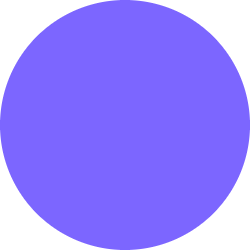
\includegraphics[scale=0.5]{images/canvas250.png}
\label{fig:Canvas2}
}
\caption[Canvas With Responsive Circles]{
Responsive rendering of graphics inside \elname{<canvas>} elements has to be
implemented manually by calculating everything relative to its dimensions. 
This figure shows the visual output
of the canvas example in Listing~\ref{list:Canvas}. 
\imgcredit{Image created by the author of this thesis.}
}
\label{fig:Canvas}
\end{figure}







\subsection{Canvas (WebGL)}
\label{sec:CanvasWebGL}

The \code{webgl} rendering context enables 3d drawing through the
WebGL version 1 API \parencite{WebGL1}. The \code{webgl2}
rendering context enables 3d drawing through the WebGL version 2 API
\parencite{WebGL2}. WebGL-based rendering is hardware-accelerated and
often much faster than rendering via a 2d canvas or SVG. It is also
possible to render 2d graphics using a WebGL render context, but the
necessary setup and rendering API is rather complex.   



\section{Layout Engines}
\label{sec:LayoutEngines}

A layout engine is used to calculate the boundary coordinates of
visual components based on input components annotated with layout
constraints. These layout constraints describe the size and position
of components and their relationships between each other in a syntax
understood by the layout engine. For browser-based layout engines, the
input components are normally declared as HTML documents, which are
constrained using CSS. More low-level layout engines require custom
formats, which usually involve a hierarchy of objects constrained
using specific properties. The most relevant layout engines in the
context of this work are summarized in the following sections.


\subsection{Browser Engines}
\label{sec:BrowserEngines}

The purpose of a browser engine is to transform document and any
additional resources, like CSS, into a visual representation. A
browser engine is a core component of every web browser, and it is
responsible for laying out elements and rendering them.  The
terminology of browser engines is ill-defined, with them sometimes
also being referred to as layout or render engines. Theoretically, the
layout and render processes could be separated into different
components, but in practice they are tightly-coupled into a combined
component, which will be referred to as a browser engine in this work.
Some notable browser engines are WebKit \parencite{WebKit}, Blink
\parencite{Blink}, and Gecko \parencite{Gecko}.

In a browser engine, the layout of elements is constrained with CSS,
which yields great flexibility as already described in
Section~\ref{sec:CSS}. A range of mechanisms is available to precisely
control the layout of elements, like the Flexible Box and Grid layout
modules, which can also be used in combination.

The layout module of a browser engine can only be invoked directly by
browsers to position HTML elements in actively rendered documents. To
use it for calculating layouts of non-HTML constructs, they must be
replicated in active documents, so they can be parsed, laid out and
rendered by the browser engine. These replicated constructs do not
necessarily have to be visible, and they could also be removed from
the document after the layout has been acquired, meaning they do not
need to be noticeable at all. A strong limitation of using browser
engines to calculate layouts is that it requires a browser runtime to
work and, even though there are solutions like Electron
\parencite{Electron} available, which enable development of desktop
applications using web technologies, this limitation forces
applications into a very specific stack of technologies.



\subsection{Yoga}
\label{sec:Yoga}

Yoga \parencite{Yoga} is a layout engine which enables the computation
of layouts constrained using the grammar defined in the CSS Flexible
Box layout module (see Section~\ref{sec:Flexbox}). It has been
maintained by Facebook as an open-source project since 2016
\parencite{YogaRelease}, with the goal of providing a small and
high-performance library which can be used across all platforms. Yoga
is implemented in C/C++, which works on a myriad of devices, with
bindings available for other platforms like JavaScript, Android, and
iOS. It has been widely adopted and is used to perform layouting in
major frameworks such as React Native \parencite{ReactNative}, Litho
\parencite{Litho}, and ComponentKit \parencite{ComponentKit}.



\subsection{FaberJS}
\label{sec:FaberJS}

FaberJS \parencite{FaberJS} is a layout engine very similar to the
Yoga layout engine in that it enables the computation of layouts for
constructs other than HTML documents, using a layout grammar
originally created for CSS. In contrast to Yoga, which is used to
create one-dimensional layouts using the Flexbox layout grammar,
FaberJS implements a two-dimensional layout algorithm built on the
grammar of the CSS Grid layout module (see Section~\ref{sec:Grid}).
This inherently two-dimensional approach to layouting is more suited
to information visualization than a one-dimensional approach. FaberJS
is an open-source JavaScript project developed since 2019 by
Idera. Even though the layouts it computes are constrained with the
Grid Layout grammar, it only supports a subset the functionality
defined in the original CSS module. Some examples of missing
functionaly include missing support for margins, gaps, and the
\cssname{*-content} and \cssname{grid-auto-*} properties. Working
around the limitations caused by these missing features is
non-trivial, and it seems unlikely that support for them will be added
by the FaberJS maintainers in the near future because, at the time of
writing, the project has not been updated in nearly two years.






\section{Responsive Web Design}
\label{sec:RWD}

Influenced by the increasing use of mobile devices and their vastly
varying screen sizes, responsive web design has established itself as
the predominant way of designing web pages. The core idea of
responsive web design is that instead of designing pages for different
types of devices, website authors create a single design for a page,
which adapts to the characteristics of the consuming device. The term
\enquote{Responsive Web Design} was initially defined by
\textcite{Marcotte-ALA-RWD} and later compiled into a book
\parencite{ResponsiveWebDesign}, in which the author differentiates
between flexible and responsive web designs. A flexible web design,
which merely fluidly scales blocks of content to make them fit into
the width of a browser window, is not enough to provide a good
experience for users. Such designs will work well enough for similarly
sized viewports to the one they were created for, but they will lead
to noticeable artifacts on lower resolutions.

These problems can be avoided by positioning the individual components
of a page in a manner which provides them with enough space to render
correctly. This can be achieved by using CSS media queries to adapt
the overall layout of a page to the dimensions of the consuming
device. Another crucial part of responsive web design is to support
the different modes of interaction inherent to the various types of
devices used to access the web. Desktop users might access a website
using a mouse, mobile device users typically interact via a
touchscreen, and yet others might consume a page in a purely textual
form with a screen reader and interact via a keyboard. It is one of
the mantras of responsive web design to provide smooth and complete
access to information to all users, regardless of the device they are
using.
